\appendix

\pagelayout{wide} % No margins
\chapter{Appendix}\label{appendix}
\def\arraystretch{1.5}
\pagelayout{margin} % Restore margins
\begin{table*}
  %\renewcommand{\arraystretch}{1.1}
  \centering
  \small
  \begin{tabular}{l r r r r c c}
    \hline
    \textbf{Event}   & \textbf{R.A. (J2000)}    & \textbf{Dec (J2000)}     & \textbf{90\% area}   & \textbf{ZTF obs}     & ~ \textbf{Signal-} & \textbf{Reference}                                    \\
                     & \textbf{(deg)}           & \textbf{(deg)}           & \textbf{(deg$^{2}$)} & \textbf{(deg$^{2}$)} & \textbf{ness}      &                                                       \\
    \hline
    \hline
    \emph{IC190503A} & $120.28^{+0.57}_{-0.77}$ & $6.35^{+0.76}_{-0.70}$   & 1.94                 & 1.37                 & \SI{36}{\percent}  & \cite{IC190503A1, IC190503A2}                         \\
    \emph{IC190619A} & $343.26^{+4.08}_{-2.63}$ & $10.73^{+1.51}_{-2.61}$  & 27.21                & 21.57                & \SI{55}{\percent}  & \cite{IC190619A1, IC190619A2}                         \\
    \emph{IC190730A} & $225.79^{+1.28}_{-1.43}$ & $10.47^{+1.14}_{-0.89}$  & 5.41                 & 4.52                 & \SI{67}{\percent}  & \cite{IC190730A1, IC190730A2}                         \\
    \emph{IC190922B} & $5.76^{+1.19}_{-1.37}$   & $-1.57^{+0.93}_{-0.82}$  & 4.48                 & 4.09                 & \SI{51}{\percent}  & \cite{IC190922B1, IC190922B2, IC190922B3}             \\
    \emph{IC191001A} & $314.08^{+6.56}_{-2.26}$ & $12.94^{+1.50}_{-1.47}$  & 25.53                & 23.06                & \SI{59}{\percent}  & \cite{IC191001A1, IC191001A2, IC191001A3}             \\
    \emph{IC200107A} & $148.18^{+2.20}_{-1.83}$ & $35.46^{+1.10}_{-1.22}$  & 7.62                 & 6.28                 & --                 & \cite{IC200107A1, IC200107A2}                         \\
    \emph{IC200109A} & $164.49^{+4.94}_{-4.19}$ & $11.87^{+1.16}_{-1.36}$  & 22.52                & 22.36                & \SI{77}{\percent}  & \cite{IC200109A1, IC200109A2}                         \\
    \emph{IC200117A} & $116.24^{+0.71}_{-1.24}$ & $29.14^{+0.90}_{-0.78}$  & 2.86                 & 2.66                 & \SI{38}{\percent}  & \cite{IC200117A1, IC200117A2, IC200117A3}             \\
    \emph{IC200512A} & $295.18^{+1.72}_{-2.26}$ & $15.79^{+1.26}_{-1.29}$  & 9.77                 & 9.26                 & \SI{32}{\percent}  & \cite{IC200512A1, IC200512A2}                         \\
    \emph{IC200530A} & $255.37^{+2.48}_{-2.56}$ & $26.61^{+2.33}_{-3.28}$  & 25.38                & 22.05                & \SI{59}{\percent}  & \cite{IC200530A1, IC200530A2, IC200530A3, IC200530A4} \\
    \emph{IC200620A} & $162.11^{+0.64}_{-0.95}$ & $11.95^{+0.63}_{-0.48}$  & 1.73                 & 1.24                 & \SI{32}{\percent}  & \cite{IC200620A1, IC200620A2}                         \\
    \emph{IC200916A} & $109.78^{+1.08}_{-1.44}$ & $14.36^{+0.88}_{-0.85}$  & 4.22                 & 3.61                 & \SI{32}{\percent}  & \cite{IC200916A1, IC200916A2, IC200916A3}             \\
    \emph{IC200926A} & $96.46^{+0.73}_{-0.55}$  & $-4.33^{+0.61}_{-0.76}$  & 1.75                 & 1.29                 & \SI{44}{\percent}  & \cite{IC200926A1, IC200926A2}                         \\
    \emph{IC200929A} & $29.53^{+0.53}_{-0.53}$  & $3.47^{+0.71}_{-0.35}$   & 1.12                 & 0.87                 & \SI{47}{\percent}  & \cite{IC200929A1, IC200929A2}                         \\
    \emph{IC201007A} & $265.17^{+0.52}_{-0.52}$ & $5.34^{+0.32}_{-0.23}$   & 0.57                 & 0.55                 & \SI{88}{\percent}  & \cite{IC201007A1, IC201007A2}                         \\
    \emph{IC201021A} & $260.82^{+1.73}_{-1.68}$ & $14.55^{+1.35}_{-0.74}$  & 6.89                 & 6.30                 & \SI{30}{\percent}  & \cite{IC201021A1, IC201021A2}                         \\
    \emph{IC201130A} & $30.54^{+1.13}_{-1.31}$  & $-12.10^{+1.15}_{-1.13}$ & 5.44                 & 4.51                 & \SI{15}{\percent}  & \cite{IC201130A1, IC201130A2}                         \\
    \emph{IC201209A} & $6.86^{+1.02}_{-1.22}$   & $-9.25^{+0.99}_{-1.14}$  & 4.71                 & 3.20                 & \SI{19}{\percent}  & \cite{IC201209A1, IC201209A2}                         \\
    \emph{IC201222A} & $206.37^{+0.90}_{-0.80}$ & $13.44^{+0.55}_{-0.38}$  & 1.54                 & 1.40                 & \SI{53}{\percent}  & \cite{IC201222A1, IC201222A2}                         \\
    \emph{IC210210A} & $206.06^{+1.40}_{-0.95}$ & $4.78^{+0.62}_{-0.56}$   & 2.76                 & 2.05                 & \SI{65}{\percent}  & \cite{IC210210A1, IC210210A2}                         \\
    \emph{IC210510A} & $268.42^{+1.47}_{-1.60}$ & $3.81^{+0.68}_{-0.64}$   & 4.04                 & 3.67                 & \SI{28}{\percent}  & \cite{IC210510A1, IC210510A2}                         \\
    \emph{IC210629A} & $340.75^{+1.11}_{-2.23}$ & $12.94^{+0.91}_{-0.93}$  & 5.99                 & 4.59                 & \SI{35}{\percent}  & \cite{IC210629A1, IC210629A2, IC210629A3}             \\
    \emph{IC210811A} & $270.79^{+1.07}_{-1.08}$ & $25.28^{+0.79}_{-0.84}$  & 3.17                 & 2.66                 & \SI{66}{\percent}  & \cite{IC210811A1, IC210811A2}                         \\
    \emph{IC210922A} & $60.73^{+0.96}_{-0.66}$  & $-4.18^{+0.42}_{-0.55}$  & 1.57                 & 1.16                 & \SI{93}{\percent}  & \cite{IC210922A1, IC210922A2}                         \\
    \emph{IC220405A} & $134.47^{+1.71}_{-1.72}$ & $-1.27^{+1.45}_{-1.02}$  & 8.47                 & 7.52                 & \SI{32}{\percent}  & \cite{IC220405A1, IC220405A2}                         \\
    \emph{IC220405B} & $320.62^{+1.37}_{-1.13}$ & $29.06^{+0.94}_{-0.68}$  & 3.54                 & 3.41                 & \SI{36}{\percent}  & \cite{IC220405B1, IC220405A2}                         \\
    \emph{IC220501A} & $311.57^{+0.82}_{-1.07}$ & $18.68^{+1.08}_{-0.92}$  & $3.58$               & 2.47                 & \SI{40}{\percent}  & \cite{IC220501A1, IC220501A2}                         \\
    \emph{IC220513A} & $224.03^{+1.36}_{-1.27}$ & $-1.34^{+0.74}_{-0.81}$  & 4.08                 & 1.93                 & \SI{56}{\percent}  & \cite{IC220513A1, IC220513A2}                         \\
    \emph{IC220624A} & $224.12^{+2.23}_{-1.95}$ & $41.31^{+1.56}_{-1.56}$  & 9.80                 & 8.09                 & \SI{61}{\percent}  & \cite{IC220624A1, IC220624A2}                         \\
    \emph{IC220822A} & $273.08^{+2.47}_{-2.50}$ & $21.54^{+0.94}_{-1.18}$  & 9.81                 & 9.63                 & \SI{38}{\percent}  & \cite{IC220822A1, IC220822A2}                         \\
    \emph{IC220907A} & $224.81^{+2.07}_{-1.95}$ & $44.7^{+0.94}_{-1.06}$   & 5.72                 & 5.41                 & \SI{46}{\percent}  & \cite{IC220907A1, IC220907A2, IC220907A3}             \\
    \emph{IC221216A} & $6.86^{+1.08}_{-2.06}$   & $10.43^{+1.54}_{-1.07}$  & 8.05                 & 5.68                 & \SI{41}{\percent}  & \cite{IC221216A1, IC221216A2}                         \\
    \emph{IC221223A} & $350.54^{+0.67}_{-0.67}$ & $34.71^{+0.67}_{-0.67}$  & 1.48                 & 0.97                 & \SI{79}{\percent}  & \cite{IC221223A1, IC221223A2}                         \\
    \emph{IC230112A} & $24.35^{+1.43}_{-1.71}$  & $0.90^{+0.63}_{-1.26}$   & 5.93                 & 5.57                 & \SI{28}{\percent}  & \cite{IC230112A1, IC230112A2}                         \\
    \hline
  \end{tabular}
  \caption[Summary of the 34 neutrino alerts followed up by ZTF]{Summary of the 34 neutrino alerts followed up by ZTF until March 2023. \textit{\SI{90}{\percent} area} indicates the rectangular localization uncertainty region as reported by IceCube. \textit{ZTF obs} indicates the area observed at least twice by ZTF, within the reported \SI{90}{\percent} localization (accounting for chip gaps). \textit{Signalness} estimates the probability that the neutrino is of astrophysical origin, rather than caused by atmospheric background (see Section~\ref{ic_event_selection}). The total followed-up area (corrected for chip gaps) is \SI{205.02}{\square\deg}.}
  \label{tab:neutrino_alert_overview}
\end{table*}

\begin{table*}
  \centering
  \def\arraystretch{1.2}
  \begin{tabular}{c c  c  c}
    \hline
    \textbf{MJD} & \textbf{Date} & \textbf{Band}     & \textbf{Flux density}  \\
                 &               & (\unit{\giga\Hz}) & (\unit{\micro\jansky}) \\
    \hline
    \hline
    58032        & 2017-11-25    & 3.00              & $\leq 320 $            \\
    59033        & 2020-07-03    & 3.00              & $ 226 \pm 13$          \\
    59033        & 2020-07-03    & 10.00             & $ 86 \pm 11$           \\
    59105        & 2020-09-13    & 1.52              & $ 390 \pm 34$          \\
    59105        & 2020-09-13    & 3.00              & $ 211 \pm 10$          \\
    59105        & 2020-09-13    & 6.00              & $ 118 \pm 6$           \\
    59105        & 2020-09-13    & 10.00             & $ 86 \pm 5$            \\
    59160        & 2020-11-07    & 1.62              & $ 373 \pm 20$          \\
    59160        & 2020-11-07    & 3.00              & $ 209 \pm 9$           \\
    59160        & 2020-11-07    & 6.00              & $ 91 \pm 6$            \\
    59160        & 2020-11-07    & 10.00             & $ 39 \pm 5$            \\
    \hline
  \end{tabular}
  \caption[AT2019fdr VLA measurements]{VLA measurements of AT2019fdr and the VLASS archival limit (first row). From~\cite{Reusch2022}.}
  \label{tab:at2019fdr_radio}
\end{table*}

\begin{table*}
  \centering
  \def\arraystretch{1.5}
  \begin{tabular}{c c c}
    \hline
    \textbf{Band}      & \textbf{$\lambda_\text{eff}$} & \textbf{AB magnitude}   \\
    \hline
    \hline
    \textit{GALEX} FUV &                               & $22.32^{+0.07}_{-0.10}$ \\
    \textit{GALEX} NUV & $21.52^{+0.06}_{-0.10}$                                 \\
    SDSS \textit{u}    & $20.91^{+0.06}_{-0.07}$                                 \\
    SDSS \textit{g}    & $19.97^{+0.04}_{-0.04}$                                 \\
    SDSS \textit{r}    & $19.00^{+0.02}_{-0.03}$                                 \\
    SDSS \textit{i}    & $18.64^{+0.02}_{-0.03}$                                 \\
    SDSS \textit{z}    & $18.36^{+0.02}_{-0.03}$                                 \\
    UKIRT \textit{J}   & $18.18 $                                                \\
    \textit{WISE W1}   & $17.83^{+0.05}_{-0.05}$                                 \\
    \textit{WISE W2}   & $17.78^{+0.03}_{-0.05}$                                 \\
    \hline
  \end{tabular}
  \caption[Archival AT2019fdr host measurements]{Archival measurements from \textit{GALEX}, SDSS, UKIRT (the isoMag value was given without error) and \textit{WISE}, used to construct the synthetic host model (see~\ref{synthetic_host_model}). From~\cite{Reusch2022}.}
  \label{tab:host_model_measurements}
\end{table*}

\begin{table*}
  \centering
  \def\arraystretch{1.5}
  \begin{tabular}{c c}
    \hline
    \textbf{Parameter}          & \textbf{Grid values}                      \\
    \hline
    \hline
    \texttt{learning\_rate}     & [\textbf{0.1}, 0.01, 0.001]               \\
    \texttt{gamma}              & [0.01, \textbf{0.1}, 0.3, 0.5, 1, 1.5, 2] \\
    \texttt{max\_depth}         & [2, 4, \textbf{7}, 10]                    \\
    \texttt{colsample\_bytree}  & [\textbf{0.3}, 0.6, 0.8, 1.0]             \\
    \texttt{subsample}          & [0.2, 0.4, 0.5, \textbf{0.6}, 0.7]        \\
    \texttt{reg\_alpha}         & [0, \textbf{0.5}, 1]                      \\
    \texttt{reg\_lambda}        & [\textbf{1}, 1.5, 2, 3, 4.5]              \\
    \texttt{min\_child\_weight} & [\textbf{1}, 3, 5, 7]                     \\
    \texttt{n\_estimators}      & [100, 250, 500, \textbf{1000}]            \\
    \hline
  \end{tabular}
  \caption[\texttt{XGBoost} hyperparameters]{\texttt{XGBoost} hyperparameter space searched and values used in the photometric classification of the nuclear sample. The value chosen for the training of the full model is shown in bold.}
  \label{tab:xgboost_grid_search}
\end{table*}

\floatsetup[longtable]{margins=centering,LTcapwidth=table} % Add this line before the longtable to increase the caption width
\begin{table*}
  \begin{tabular}{l  c  c  c   c  c  c}
    \hline
    \textbf{Transient}                                                                                & \textbf{z}          & \textbf{z}                          & \textbf{Community}      & \textbf{IAU name}                                                 & \textbf{Peak mag.}         & \textbf{Notes}           \\
                                                                                                      &                     & \textbf{type}                       & \textbf{classification} &                                                                   & \textbf{(\textit{g}-band)} &                          \\
    \hline
    \hline
    \textit{\href{https://ztfnuclear.simeonreusch.com/transient/ZTF17aaazdba}{ZTF17aaazdba}}          & 0.022               & spec.                               & TDE                     &
    \textit{\href{https://www.wis-tns.org/object/2019azh}{AT2019azh} }                                & 15.3                &                                                                                                                                                                                           \\
    \textit{\href{https://ztfnuclear.simeonreusch.com/transient/ZTF18aakelin}{ZTF18aakelin}}          & 0.071               & spec.                               & TDE                     &
    \textit{\href{https://www.wis-tns.org/object/2020ocn}{AT2020ocn}}                                 & 19.5                &                                                                                                                                                                                           \\
    \textbf{\textit{\href{https://ztfnuclear.simeonreusch.com/transient/ZTF18abtnfnq}{ZTF18abtnfnq}}} & \textbf{0.131}      & \textbf{phot.}                      & ~                       & ~                                                                 & \textbf{20.3}              & \textbf{Large dust echo} \\
    \textit{\href{https://ztfnuclear.simeonreusch.com/transient/ZTF18abtnfnq}{ZTF18abxftqm}}          & 0.108               & phot.                               & TDE                     &
    \textit{\href{https://www.wis-tns.org/object/2018hco}{AT2018hco}}                                 & 18.3                &                                                                                                                                                                                           \\

    \textit{\href{https://ztfnuclear.simeonreusch.com/transient/ZTF18acaqdaa}{ZTF18acaqdaa}}          & 0.203               & spec.                               & TDE                     &
    \textit{\href{https://www.wis-tns.org/object/2018iih}{AT2018iih}}                                 & 18.3                &                                                                                                                                                                                           \\
    \textit{\href{https://ztfnuclear.simeonreusch.com/transient/ZTF18acbwomm}{ZTF18acbwomm}}
                                                                                                      & 0.137               & phot.                               & AGN                     & ~                                                                 & 19.2                       &                          \\
    \textit{\href{https://ztfnuclear.simeonreusch.com/transient/ZTF18accttxu}{ZTF18accttxu}}          & ~                   & ~                                   & ~                       &
    \textit{\href{https://www.wis-tns.org/object/2018lyq}{AT2018lyq}}                                 & 19.7                &                                                                                                                                                                                           \\
    \textit{\href{https://ztfnuclear.simeonreusch.com/transient/ZTF18accvmgs}{ZTF18accvmgs}}          & ~                   & ~                                   & ~                       &
    \textbf{\textit{\href{https://www.wis-tns.org/object/2018ibg}{AT2018ibg}}}                        & \textbf{19.9      } &                                                                                                                                                                                           \\
    \textit{\href{https://ztfnuclear.simeonreusch.com/transient/ZTF18acetnxh}{ZTF18acetnxh}}
                                                                                                      & 0.101               & phot.                               & Blazar                  &
    \textit{\href{https://www.wis-tns.org/object/2016fqa}{AT2016fqa}}                                 & 18.6                &                                                                                                                                                                                           \\
    \textit{\href{https://ztfnuclear.simeonreusch.com/transient/ZTF18acqighv}{ZTF18acqighv}}          & ~                   & ~                                   & AGN                     &
    \textit{\href{https://www.wis-tns.org/object/2019afh}{AT2019afh}}                                 & 19.3                &                                                                                                                                                                                           \\
    \textit{\href{https://ztfnuclear.simeonreusch.com/transient/ZTF18actaqdw}{ZTF18actaqdw}}          & ~                   & ~                                   & TDE                     &
    \textit{\href{https://www.wis-tns.org/object/2018lni}{AT2018lni}}                                 & 19.2                &                                                                                                                                                                                           \\
    \textbf{\textit{\href{https://ztfnuclear.simeonreusch.com/transient/ZTF19aaeukyu}{ZTF19aaeukyu}}} & ~                   & ~                                   & ~                       &
    \textbf{\textit{\href{https://www.wis-tns.org/object/2021aatf}{AT2021aatf}}}                      & \textbf{19.2}       &                                                                                                                                                                                           \\
    \textit{\href{https://ztfnuclear.simeonreusch.com/transient/ZTF19aaniqrr}{ZTF19aaniqrr}}
                                                                                                      & ~                   & ~                                   & TDE                     &
    \textit{\href{https://www.wis-tns.org/object/2019cmw}{AT2019cmw}}                                 & 18.5                &                                                                                                                                                                                           \\
    \textit{\href{https://ztfnuclear.simeonreusch.com/transient/ZTF19aanlttm}{ZTF19aanlttm}}          & ~                   & ~                                   & ~                       &
    \textbf{\textit{\href{https://www.wis-tns.org/object/2019cyt}{AT2019cyt}}}                        & \textbf{19.2}       &                                                                                                                                                                                           \\
    \textit{\href{https://ztfnuclear.simeonreusch.com/transient/ZTF19aapreis}{ZTF19aapreis}}
                                                                                                      & ~                   & ~                                   & TDE                     & \textit{\href{https://www.wis-tns.org/object/2019dsg}{AT2019dsg}} & 17.8                       &                          \\
    \textbf{\textit{\href{https://ztfnuclear.simeonreusch.com/transient/ZTF19aaprhvf}{ZTF19aaprhvf}}} & ~                   & ~                                   & ~                       &
    \textbf{\textit{\href{https://www.wis-tns.org/object/2019ekr}{AT2019ekr}}}                        & \textbf{19.1}       &                                                                                                                                                                                           \\
    \textbf{\textit{\href{https://ztfnuclear.simeonreusch.com/transient/ZTF19aayvxgy}{ZTF19aayvxgy}}}
                                                                                                      & ~                   & ~                                   & ~                       & ~                                                                 & \textbf{19.7}              &                          \\

    \textit{\href{https://ztfnuclear.simeonreusch.com/transient/ZTF19aaywayr}{ZTF19aaywayr}}          & ~                   & ~                                   & ~                       & ~                                                                 & 18.2                       & Evolution too slow       \\
    \textbf{\textit{\href{https://ztfnuclear.simeonreusch.com/transient/ZTF19aazlrsy}{ZTF19aazlrsy}}} & ~                   & ~                                   & AGN                     &
    \textbf{\textit{\href{https://www.wis-tns.org/object/2019hrg}{AT2019hrg}}}                        & \textbf{ 19.2}      & \textbf{Could also be AGN activity}                                                                                                                                                       \\
    \textit{\href{https://ztfnuclear.simeonreusch.com/transient/ZTF19abhejal}{ZTF19abhejal}}          & 0.200               & phot.                               & TDE                     &
    \textit{\href{https://www.wis-tns.org/object/2019mha}{AT2019mha}}                                 & 19.3                &                                                                                                                                                                                           \\
    \textit{\href{https://ztfnuclear.simeonreusch.com/transient/ZTF19abhhjcc}{ZTF19abhhjcc}}          & 0.204               & phot.                               & TDE                     &
    \textit{\href{https://www.wis-tns.org/object/2019meg}{AT2019meg}}                                 & 19.2                &                                                                                                                                                                                           \\
    \textit{\href{https://ztfnuclear.simeonreusch.com/transient/ZTF19abicvxs}{ZTF19abicvxs}}          & ~                   & ~                                   & ~                       & ~                                                                 & 19.9                       &                          \\
    \textit{\href{https://ztfnuclear.simeonreusch.com/transient/ZTF19ablizhi}{ZTF19ablizhi}}          & ~                   & ~                                   & ~                       & ~                                                                 & 19.8                       &                          \\
    \textbf{\textit{\href{https://ztfnuclear.simeonreusch.com/transient/ZTF19abqyosy}{ZTF19abqyosy}}} & \textbf{0.183}      & \textbf{phot.}                      & ~                       & ~                                                                 & \textbf{19.8}              & \textbf{Large dust echo} \\
    \textbf{\textit{\href{https://ztfnuclear.simeonreusch.com/transient/ZTF19abrbskk}{ZTF19abrbskk}}} & \textbf{0.504}      & \textbf{spec.}                      & ~                       &
    \textbf{\textit{\href{https://www.wis-tns.org/object/2019pcl}{AT2019pcl}}}                        & \textbf{18.8}       & \textbf{Very bright}                                                                                                                                                                      \\
    \textbf{\textit{\href{https://ztfnuclear.simeonreusch.com/transient/ZTF19abzzuef}{ZTF19abzzuef}}} & ~                   & ~                                   & ~                       &
    \textbf{\textit{\href{https://www.wis-tns.org/object/2019sez}{AT2019sez}}}                        & \textbf{19.5}       &                                                                                                                                                                                           \\
    \textit{\href{https://ztfnuclear.simeonreusch.com/transient/ZTF19acanuza}{ZTF19acanuza}}          & 0.167               & spec.                               & AGN                     & ~                                                                 & 19.5                       &                          \\
    \textbf{\textit{\href{https://ztfnuclear.simeonreusch.com/transient/ZTF19aclocml}{ZTF19aclocml}}} & ~                   & ~                                   & ~                       & ~                                                                 & \textbf{19.7}              &                          \\
    \textit{\href{https://ztfnuclear.simeonreusch.com/transient/ZTF19acspeuw}{ZTF19acspeuw}}          & 0.134               & phot.                               & TDE                     &
    \textit{\href{https://www.wis-tns.org/object/2019vcb}{AT2019vcb}}                                 & 18.4                &                                                                                                                                                                                           \\
    \textbf{\textit{\href{https://ztfnuclear.simeonreusch.com/transient/ZTF19acssksf}{ZTF19acssksf}}} & ~                   & ~                                   & \textbf{ AGN?}          &
    \textbf{\textit{\href{https://www.wis-tns.org/object/2019uyn}{AT2019uyn}}}                        & \textbf{19.1}       &                                                                                                                                                                                           \\
    \textit{\href{https://ztfnuclear.simeonreusch.com/transient/ZTF20aabqihu}{ZTF20aabqihu}}          & 0.070               & phot.                               & TDE                     &
    \textit{\href{https://www.wis-tns.org/object/2020pj}{AT2020pj}}                                   & 18.7                &                                                                                                                                                                                           \\
    \textbf{\textit{\href{https://ztfnuclear.simeonreusch.com/transient/ZTF20aavoumq}{ZTF20aavoumq}}} & \textbf{0.186}      & \textbf{phot.}                      &
    \textbf{AGN?}                                                                                     & ~                   & \textbf{19.5}                       &                                                                                                                                                     \\
    \textbf{\textit{\href{https://ztfnuclear.simeonreusch.com/transient/ZTF20abbpxut}{ZTF20abbpxut}}} & \textbf{0.18}       & \textbf{spec.}                      & \textbf{AGN?}           &
    \textbf{\textit{\href{https://www.wis-tns.org/object/2020kri}{AT2020kri}}}                        & \textbf{18.9}       &                                                                                                                                                                                           \\
    \textit{\href{https://ztfnuclear.simeonreusch.com/transient/ZTF20abefeab}{ZTF20abefeab}}          & 0.157               & phot.                               & TDE                     &
    \textit{\href{https://www.wis-tns.org/object/2020mbq}{AT2020mbq}}                                 & 18.8                &                                                                                                                                                                                           \\
    \textit{\href{https://ztfnuclear.simeonreusch.com/transient/ZTF20abfcszi}{ZTF20abfcszi}}          & ~                   & ~                                   & TDE                     &
    \textit{\href{https://www.wis-tns.org/object/2020mot}{AT2020mot}}                                 & 18.2                &                                                                                                                                                                                           \\
  \end{tabular}
  \caption[Final TDE (candidates)]{Curated final list of TDE candidates as classified by \texttt{XGBoost}, appended with redshifts and community classifications from Fritz, the GROWTH Marshal and TNS. All objects previously unclassified and compatible with a TDE interpretation after visual inspection and manual cross checking are shown in bold (i.e.~the new candidates).}
  \label{tab:tde_candidates}
\end{table*}

\begin{table*}
  \begin{tabular}{l  c  c  c   c  c  c}
    \hline
    \textbf{Transient}                                                                                & \textbf{z}     & \textbf{z}     & \textbf{Community}      & \textbf{IAU name} & \textbf{Peak mag.}         & \textbf{Notes}       \\
                                                                                                      &                & \textbf{type}  & \textbf{classification} &                   & \textbf{(\textit{g}-band)} &                      \\
    \hline
    \hline
    \textit{\href{https://ztfnuclear.simeonreusch.com/transient/ZTF20abjbkgq}{ZTF20abjbkgq}}          & 0.349          & phot.          & AGN                     &
    \textit{\href{https://www.wis-tns.org/object/2020qmx}{AT2020qmx}}                                 & 19.4           &                                                                                                                  \\
    \textit{\href{https://ztfnuclear.simeonreusch.com/transient/ZTF20abjwvae}{ZTF20abjwvae}}          & 0.200          & phot.          & TDE                     &
    \textit{\href{https://www.wis-tns.org/object/2020opy}{AT2020opy}}                                 & 18.9           &                                                                                                                  \\
    \textbf{\textit{\href{https://ztfnuclear.simeonreusch.com/transient/ZTF20abkstjk}{ZTF20abkstjk}}} & ~              & ~              & ~                       & ~                 & \textbf{19.2}              &                      \\
    \textit{\href{https://ztfnuclear.simeonreusch.com/transient/ZTF20abnorit}{ZTF20abnorit}}          & 0.296          & phot.          & TDE                     &
    \textit{\href{https://www.wis-tns.org/object/2020ysg}{AT2020ysg}}                                 & 18.6           &                                                                                                                  \\
    \textit{\href{https://ztfnuclear.simeonreusch.com/transient/ZTF20abowque}{ZTF20abowque}}          & 0.333          & phot.          & TDE                     &
    \textit{\href{https://www.wis-tns.org/object/2020qhs}{AT2020qhs}}                                 & 18.9           &                                                                                                                  \\
    \textbf{\textit{\href{https://ztfnuclear.simeonreusch.com/transient/ZTF20abqjebg}{ZTF20abqjebg}}} & \textbf{0.113} & \textbf{phot.} & ~                       & ~                 & \textbf{19.3}              &                      \\
    \textit{\href{https://ztfnuclear.simeonreusch.com/transient/ZTF20absxcuv}{ZTF20absxcuv}}          & ~              & ~              & ~                       & ~                 & 18.6                       &                      \\
    \textbf{\textit{\href{https://ztfnuclear.simeonreusch.com/transient/ZTF20acfxnyr}{ZTF20acfxnyr}}} & \textbf{0.127} & \textbf{phot.} & ~                       & ~                 & \textbf{19.8}              &                      \\
    \textit{\href{https://ztfnuclear.simeonreusch.com/transient/ZTF20achpcvt}{ZTF20achpcvt}}          & 0.033          & spec.          & TDE                     &
    \textit{\href{https://www.wis-tns.org/object/2020vwl}{AT2020vwl}}                                 & 17.6           &                                                                                                                  \\
    \textit{\href{https://ztfnuclear.simeonreusch.com/transient/ZTF20achupkw}{ZTF20achupkw}}          & 0.325          & phot.          & IIn                     &
    \textit{\href{https://www.wis-tns.org/object/2020vws}{SN2020vws}}                                 & 19.2           &                                                                                                                  \\
    \textbf{\textit{\href{https://ztfnuclear.simeonreusch.com/transient/ZTF20aclgfji}{ZTF20aclgfji}}} & \textbf{0.134} & \textbf{spec.} & ~                       &
    \textbf{\textit{\href{https://www.wis-tns.org/object/2020ygl}{AT2020ygl}}}                        & \textbf{19.3}  &                                                                                                                  \\
    \textit{\href{https://ztfnuclear.simeonreusch.com/transient/ZTF20acllkua}{ZTF20acllkua}}          & 0.241          & phot.          & ~                       & ~                 & 20.2                       & Evolving too fast    \\
    \textit{\href{https://ztfnuclear.simeonreusch.com/transient/ZTF20acnznms}{ZTF20acnznms}}          & 0.203          & phot.          & SLSN-II                 &
    \textit{\href{https://www.wis-tns.org/object/2020yue}{SN2020yue}}                                 & 18.5           &                                                                                                                  \\
    \textbf{\textit{\href{https://ztfnuclear.simeonreusch.com/transient/ZTF20acpmkls}{ZTF20acpmkls}}} & \textbf{0.072} & \textbf{spec.} & ~                       & ~                 & \textbf{19.9}              &                      \\
    \textit{\href{https://ztfnuclear.simeonreusch.com/transient/ZTF20acwytxn}{ZTF20acwytxn}}          & 0.319          & phot.          & TDE                     &
    \textit{\href{https://www.wis-tns.org/object/2020acka}{AT2020acka}}                               & 18.1           &                                                                                                                  \\
    \textit{\href{https://ztfnuclear.simeonreusch.com/transient/ZTF20acyydkh}{ZTF20acyydkh}}          & 0.127          & phot.          & TDE                     &
    \textit{\href{https://www.wis-tns.org/object/2021ack}{AT2021ack}}                                 & 19.1           &                                                                                                                  \\
    \textit{\href{https://ztfnuclear.simeonreusch.com/transient/ZTF21aabgjcz}{ZTF21aabgjcz}}          & ~              & ~              & TDE                     &
    \textit{\href{https://www.wis-tns.org/object/2020aexc}{AT2020aexc}}                               & 19.2           &                                                                                                                  \\
    \textit{\href{https://ztfnuclear.simeonreusch.com/transient/ZTF21aabiipy}{ZTF21aabiipy}}          & 0.278          & phot.          & TDE                     &
    \textit{\href{https://www.wis-tns.org/object/2021lo}{AT2021lo}}                                   & 19.2           &                                                                                                                  \\
    \textit{\href{https://ztfnuclear.simeonreusch.com/transient/ZTF21aaeoitd}{ZTF21aaeoitd}}          & 0.151          & phot.          & TDE                     &
    \textit{\href{https://www.wis-tns.org/object/2021jsg}{AT2021jsg}}                                 & 19.5           &                                                                                                                  \\
    \textit{\href{https://ztfnuclear.simeonreusch.com/transient/ZTF21aakfqwq}{ZTF21aakfqwq}}          & 0.117          & phot.          & TDE                     &
    \textit{\href{https://www.wis-tns.org/object/2021crk}{AT2021crk}}                                 & 19.1           &                                                                                                                  \\
    \textit{\href{https://ztfnuclear.simeonreusch.com/transient/ZTF21aalydww}{ZTF21aalydww}}          & 0.189          & phot.          & ~                       & ~                 & 19.4                       &                      \\
    \textbf{\textit{\href{https://ztfnuclear.simeonreusch.com/transient/ZTF21aanubdr}{ZTF21aanubdr}}} & ~              & ~              & ~                       & ~                 & \textbf{19.3}              & \textbf{Little data} \\
    \textit{\href{https://ztfnuclear.simeonreusch.com/transient/ZTF21aaqgbln}{ZTF21aaqgbln}}          & ~              & ~              & ~                       & ~                 & 19.5                       &                      \\
    \textbf{\textit{\href{https://ztfnuclear.simeonreusch.com/transient/ZTF21aaxtlvc}{ZTF21aaxtlvc}}} & \textbf{0.161} & \textbf{phot.} & ~                       &
    \textbf{\textit{\href{https://www.wis-tns.org/object/2021ldl}{AT2021ldl}}}                        & \textbf{19.6 } &                                                                                                                  \\
    \textbf{\textit{\href{https://ztfnuclear.simeonreusch.com/transient/ZTF21aaxtpty}{ZTF21aaxtpty}}} & \textbf{0.126} & \textbf{phot.} & ~                       &
    \textbf{\textit{\href{https://www.wis-tns.org/object/2021kqp}{AT2021kqp}}}                        & \textbf{19.1}  &                                                                                                                  \\
    \textit{\href{https://ztfnuclear.simeonreusch.com/transient/ZTF21aaxxyha}{ZTF21aaxxyha}}          & 0.166          & spec.          & ~                       &
    \textit{\href{https://www.wis-tns.org/object/2021kuk}{AT2021kuk}}                                 & 19.3           &                                                                                                                  \\
    \textbf{\textit{\href{https://ztfnuclear.simeonreusch.com/transient/ZTF21aazenvp}{ZTF21aazenvp}}} & \textbf{0.213} & \textbf{phot.} & ~                       &
    \textbf{\textit{\href{https://www.wis-tns.org/object/2021ovg}{AT2021ovg}}}                        & \textbf{20.0}  &                                                                                                                  \\
    \textit{\href{https://ztfnuclear.simeonreusch.com/transient/ZTF21aazewul}{ZTF21aazewul}}          & ~              & ~              & ~                       &
    \textit{\href{https://www.wis-tns.org/object/2021uwm}{AT2021uwm}}                                 & 19.3           &                                                                                                                  \\
    \textit{\href{https://ztfnuclear.simeonreusch.com/transient/ZTF21abcgnqn}{ZTF21abcgnqn}}          & 0.047          & spec.          & TDE                     &
    \textit{\href{https://www.wis-tns.org/object/2021nwa}{AT2021nwa}}                                 & 18.4           &                                                                                                                  \\
    \textit{\href{https://ztfnuclear.simeonreusch.com/transient/ZTF21abjrysr}{ZTF21abjrysr}}          & ~              & ~              & TDE                     &
    \textit{\href{https://www.wis-tns.org/object/2021sdu}{AT2021sdu}}                                 & 11.6           &                                                                                                                  \\
    \textbf{\textit{\href{https://ztfnuclear.simeonreusch.com/transient/ZTF21abkqvdo}{ZTF21abkqvdo}}} & \textbf{0.096} & \textbf{phot.} & ~                       &
    \textbf{\textit{\href{https://www.wis-tns.org/object/2021swi}{AT2021swi}}}                        & \textbf{18.8}  &                                                                                                                  \\
    \textit{\href{https://ztfnuclear.simeonreusch.com/transient/ZTF21abqhkjd}{ZTF21abqhkjd}}          & 0.131          & phot.          & TDE                     &
    \textit{\href{https://www.wis-tns.org/object/2021uqv}{AT2021uqv}}                                 & 18.9           &                                                                                                                  \\
    \textit{\href{https://ztfnuclear.simeonreusch.com/transient/ZTF21absltzp}{ZTF21absltzp}}          & 0.086          & phot.          & ~                       &
    \textit{\href{https://www.wis-tns.org/object/2021vvw}{AT2021vvw}}                                 & 19.3           &                                                                                                                  \\
    \textit{\href{https://ztfnuclear.simeonreusch.com/transient/ZTF21acafvhf}{ZTF21acafvhf}}          & ~              & ~              & TDE                     &
    \textit{\href{https://www.wis-tns.org/object/2021yte}{AT2021yte}}                                 & 18.7           &                                                                                                                  \\
    \textit{\href{https://ztfnuclear.simeonreusch.com/transient/ZTF21acdsrxc}{ZTF21acdsrxc}}          & 0.081          & spec.          & ~                       & ~                 & 19.2                       &                      \\
    \textit{\href{https://ztfnuclear.simeonreusch.com/transient/ZTF21achnqdo}{ZTF21achnqdo}}          & ~              & ~              & ~                       &
    \textit{\href{https://www.wis-tns.org/object/2021aczv}{AT2021aczv}}                               & 19.9           &                                                                                                                  \\
  \end{tabular}
\end{table*}

\begin{table*}[t!]
  \begin{tabular}{l  c  c  c  c  c  c}
    \hline
    \textbf{Transient}                                                           & \textbf{z}     & \textbf{z}     & \textbf{Community}      & \textbf{IAU name} & \textbf{Peak mag.}         & \textbf{Notes} \\
                                                                                 &                & \textbf{type}  & \textbf{classification} &                   & \textbf{(\textit{g}-band)} &                \\
    \hline
    \hline
    \textbf{\textit{ZTF21acojhgu}}                                               & \textbf{0.290} & \textbf{phot.} & ~                       &
    \textbf{\textit{\href{https://www.wis-tns.org/object/2021aees}{AT2021aees}}} & \textbf{18.7}  &                                                                                                            \\
    \textit{ZTF22aaabovl}                                                        & 0.137          & phot.          & TDE                     &
    \textit{\href{https://www.wis-tns.org/object/2022aee}{AT2022aee}}            & 18.3           &                                                                                                            \\
    \textbf{\textit{ZTF22aaabqko}}                                               & \textbf{0.087} & \textbf{phot.} & ~                       &
    \textbf{\textit{\href{https://www.wis-tns.org/object/2022emf}{AT2022emf}}}   & \textbf{19.7}  &                                                                                                            \\
    \textit{ZTF22aaaedas}                                                        & 0.186          & phot.          & TDE                     &
    \textit{\href{https://www.wis-tns.org/object/2022rz}{AT2022rz}}              & 18.9           &                                                                                                            \\
    \textit{ZTF22aaahtqz}                                                        & 0.038          & spec.          & TDE                     &
    \textit{\href{https://www.wis-tns.org/object/2022bdw}{AT2022bdw}}            & 17.4           &                                                                                                            \\
    \textit{ZTF22aabimec}                                                        & 0.210          & phot.          & Ic-SLSN                 &
    \textit{\href{https://www.wis-tns.org/object/2022csn}{AT2022csn}}            & 18.5           &                                                                                                            \\
    \textit{ZTF22aacgcwv}                                                        & 0.072          & spec.          & TDE                     &
    \textit{\href{https://www.wis-tns.org/object/2022dyt}{AT2022dyt}}            & 19.7           &                                                                                                            \\
    \textit{ZTF22aaddwbo}                                                        & 0.145          & phot.          & TDE                     &
    \textit{\href{https://www.wis-tns.org/object/2022gdw}{AT2022gdw}}            & 19.0           &                                                                                                            \\
    \hline
  \end{tabular}
\end{table*}


% \caption[Final dust echo selection)]{Final list of nuclear sample transients showing strong dust echoes. All transients listed here passed a visual selection by at least two persons.}
% \label{tab:dustecho_selection}









\begin{table*}[t!]
  \resizebox{1.5\textwidth}{!}{%
    \begin{tabular}{c  c  c  c  c  c  c  c}
      \hline
      \textbf{Light curve}                                                                                                                        & \textbf{Transient}                                                                                & \textbf{z}                     & \textbf{z}     & \textbf{Community}      & \textbf{IAU name}                                                          & \textbf{Peak mag.}         & \textbf{Notes}            \\
                                                                                                                                                  &                                                                                                   &                                & \textbf{type}  & \textbf{classification} &                                                                            & \textbf{(\textit{g}-band)} &                           \\
      \hline
      \hline
      \parbox[c]{12em}{\includegraphics[width=0.4\textwidth]{/Users/simeon/ZTFDATA/nuclear_sample/plots/lightcurves/thumbnails/ZTF18aajupnt.pdf}} & \textit{\href{https://ztfnuclear.simeonreusch.com/transient/ZTF18aajupnt}{ZTF18aajupnt}}          & 0.037                          & spec.          & CLAGN                   &
      \textit{\href{https://www.wis-tns.org/object/2018dyk}{AT2018dyk}}                                                                           & 18.58                                                                                             & \cite{Frederick2019,Huang2023}                                                                                                                                                                                  \\
      \parbox[c]{12em}{\includegraphics[width=0.4\textwidth]{/Users/simeon/ZTFDATA/nuclear_sample/plots/lightcurves/thumbnails/ZTF18abjjkeo.pdf}} & \textit{\href{https://ztfnuclear.simeonreusch.com/transient/ZTF18abjjkeo}{ZTF18abjjkeo}}          & 0.103                          & spec.          & NLSy1 accr. flare       &
      \textit{\href{https://www.wis-tns.org/object/2020hle}{AT2020hle}}                                                                           & 18.65                                                                                             & \cite{Frederick2021}                                                                                                                                                                                            \\
      \parbox[c]{12em}{\includegraphics[width=0.4\textwidth]{/Users/simeon/ZTFDATA/nuclear_sample/plots/lightcurves/thumbnails/ZTF18abnwufa.pdf}} & \textbf{\textit{\href{https://ztfnuclear.simeonreusch.com/transient/ZTF18abnwufa}{ZTF18abnwufa}}} & \textbf{0.124}                 & \textbf{phot.} & \textbf{Unclassified}   & ~                                                                          & \textbf{19.76}             &                           \\
      \parbox[c]{12em}{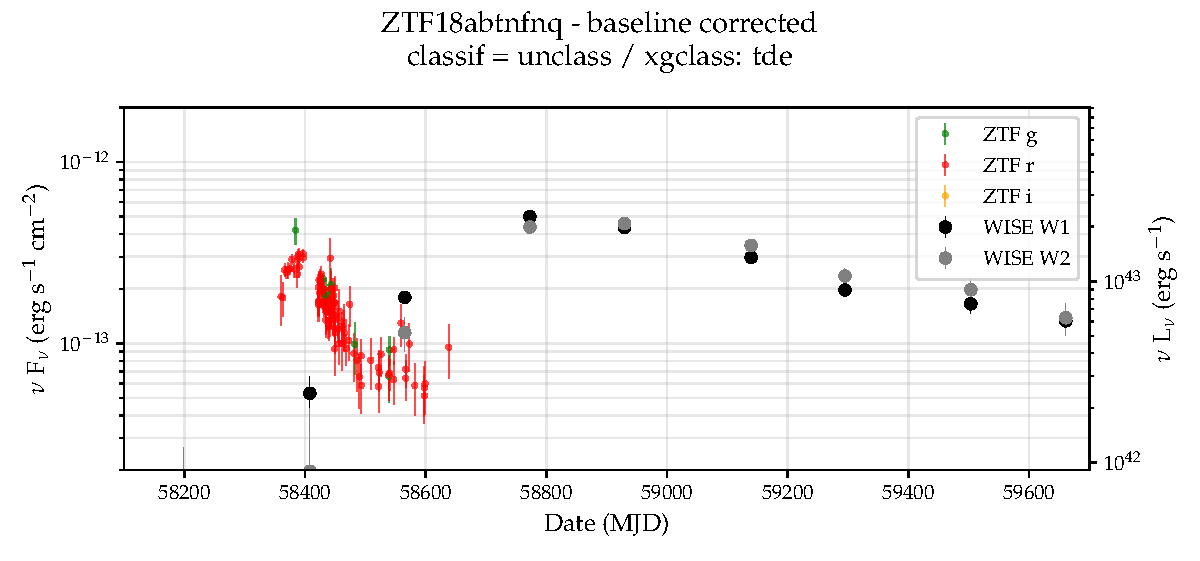
\includegraphics[width=0.4\textwidth]{/Users/simeon/ZTFDATA/nuclear_sample/plots/lightcurves/thumbnails/ZTF18abtnfnq.pdf}} & \textbf{\textit{\href{https://ztfnuclear.simeonreusch.com/transient/ZTF18abtnfnq}{ZTF18abtnfnq}}} & \textbf{0.131}                 & \textbf{phot.} & \textbf{Unclassified}   & ~                                                                          & \textbf{20.26}             &                           \\
      \parbox[c]{12em}{\includegraphics[width=0.4\textwidth]{/Users/simeon/ZTFDATA/nuclear_sample/plots/lightcurves/thumbnails/ZTF18acgqweq.pdf}} & \textit{\href{https://ztfnuclear.simeonreusch.com/transient/ZTF18acgqweq}{ZTF18acgqweq}}          & 0.167                          & spec.          & AGN                     & \textit{\href{https://www.wis-tns.org/object/2018iql}{AT2018iql}}          & 18.25                      & \cite{Velzen2021}         \\
      \parbox[c]{12em}{\includegraphics[width=0.4\textwidth]{/Users/simeon/ZTFDATA/nuclear_sample/plots/lightcurves/thumbnails/ZTF18adbifqw.pdf}} & \textit{\href{https://ztfnuclear.simeonreusch.com/transient/ZTF18adbifqw}{ZTF18adbifqw}}          & 0.121                          & phot.          & Unclassified            & \textit{\href{https://www.wis-tns.org/object/2018lhv}{AT2018lhv}}          & 19.14                      & \cite{Velzen2021}         \\
      \parbox[c]{12em}{\includegraphics[width=0.4\textwidth]{/Users/simeon/ZTFDATA/nuclear_sample/plots/lightcurves/thumbnails/ZTF19aailpwl.pdf}} & \textit{\href{https://ztfnuclear.simeonreusch.com/transient/ZTF19aailpwl}{ZTF19aailpwl}}          & 0.374                          & spec.          & various                 & \textit{\href{https://www.wis-tns.org/object/2019brs}{AT2019brs}}          & 18.24                      & $\mu$TDE?~\cite{Yang2022} \\
      \parbox[c]{12em}{\includegraphics[width=0.4\textwidth]{/Users/simeon/ZTFDATA/nuclear_sample/plots/lightcurves/thumbnails/ZTF19aakrnwh.pdf}} & \textit{\href{https://ztfnuclear.simeonreusch.com/transient/ZTF19aakrnwh}{ZTF19aakrnwh}}          & 0.285                          & phot.          & \textbf{Unclassified}   & \textit{\href{https://www.wis-tns.org/object/2021aeuf}{AT2021aeuf}}        & 18.26                      & \cite{Velzen2021}         \\
      \parbox[c]{12em}{\includegraphics[width=0.4\textwidth]{/Users/simeon/ZTFDATA/nuclear_sample/plots/lightcurves/thumbnails/ZTF19aamsgro.pdf}} & \textbf{\textit{\href{https://ztfnuclear.simeonreusch.com/transient/ZTF19aamsgro}{ZTF19aamsgro}}} & \textbf{0.262}                 & \textbf{spec.} & \textbf{AGN}            & \textbf{\textit{\href{https://www.wis-tns.org/object/2019cyq}{AT2019cyq}}} & \textbf{18.5}              & \textbf{CLAGN?}           \\
    \end{tabular}}
  \caption[Dust echo selection]{Curated list of ZTF nuclear sample transients displaying strong \textit{WISE}-detected infrared dust echoes. All transients listed here passed a visual selection by at least two persons. Sources in bold are newly published in this work. Several sources were already published in~\ref{Velzen2021}, as a comparable metric to identify dust echoes was employed. All light curve plots show a time range of 3 years, and the flux ranges between \num{2e-14} and \SI{8e-12}{\erg\per\s\per\cm\squared}.}
  \label{tab:dustecho_selection}
\end{table*}


\begin{table*}[t!]
  \resizebox{1.5\textwidth}{!}{%
    \begin{tabular}{c  c  c  c  c  c  c  c}
      \hline
      \textbf{Light curve}                                                                                                                        & \textbf{Transient}                                                                       & \textbf{z} & \textbf{z}      & \textbf{Community}      & \textbf{IAU name}                                                   & \textbf{Peak mag.}         & \textbf{Notes}                      \\
                                                                                                                                                  &                                                                                          &            & \textbf{type}   & \textbf{classification} &                                                                     & \textbf{(\textit{g}-band)} &                                     \\
      \hline
      \hline
      \parbox[c]{12em}{\includegraphics[width=0.4\textwidth]{/Users/simeon/ZTFDATA/nuclear_sample/plots/lightcurves/thumbnails/ZTF19aapreis.pdf}} & \textit{\href{https://ztfnuclear.simeonreusch.com/transient/ZTF19aapreis}{ZTF19aapreis}} & 0.051      & spec.           & TDE                     & \textit{\href{https://www.wis-tns.org/object/2019dsg}{AT2019dsg}}   & 17.8                       & See Section~\ref{at2019dsg}         \\
      \parbox[c]{12em}{\includegraphics[width=0.4\textwidth]{/Users/simeon/ZTFDATA/nuclear_sample/plots/lightcurves/thumbnails/ZTF19aasnaqa.pdf}} & \textit{\href{https://ztfnuclear.simeonreusch.com/transient/ZTF19aasnaqa}{ZTF19aasnaqa}} & 0.298      & spec. by author & Unclassified            & \textit{\href{https://www.wis-tns.org/object/2019gur}{AT2019gur}}   & 19.74                      & \cite{Velzen2021}                   \\
      \parbox[c]{12em}{\includegraphics[width=0.4\textwidth]{/Users/simeon/ZTFDATA/nuclear_sample/plots/lightcurves/thumbnails/ZTF19aatubsj.pdf}} & \textit{\href{https://ztfnuclear.simeonreusch.com/transient/ZTF19aatubsj}{ZTF19aatubsj}} & 0.266      & spec.           & accretion flare         & \textit{\href{https://www.wis-tns.org/object/2019fdr}{AT2019fdr}}   & 18.12                      & See Chapter~\ref{at2019fdr}         \\
      \parbox[c]{12em}{\includegraphics[width=0.4\textwidth]{/Users/simeon/ZTFDATA/nuclear_sample/plots/lightcurves/thumbnails/ZTF19aaujlpo.pdf}} & \textit{\href{https://ztfnuclear.simeonreusch.com/transient/ZTF19aaujlpo}{ZTF19aaujlpo}} & 0.054      & spec.           & Unclassified            & \textit{\href{https://www.wis-tns.org/object/2019idm}{AT2019idm}}   & 19.21                      & \cite{Velzen2021}, X-ray detection! \\
      \parbox[c]{12em}{\includegraphics[width=0.4\textwidth]{/Users/simeon/ZTFDATA/nuclear_sample/plots/lightcurves/thumbnails/ZTF19aavihif.pdf}} & \textit{\href{https://ztfnuclear.simeonreusch.com/transient/ZTF19aavihif}{ZTF19aavihif}} & 0.212      & phot.           & AGN                     & \textit{\href{https://www.wis-tns.org/object/2019hbh}{AT2019hbh}}   & 19.45                      & \cite{Velzen2021}                   \\
      \parbox[c]{12em}{\includegraphics[width=0.4\textwidth]{/Users/simeon/ZTFDATA/nuclear_sample/plots/lightcurves/thumbnails/ZTF19aavprgm.pdf}} & \textit{\href{https://ztfnuclear.simeonreusch.com/transient/ZTF19aavprgm}{ZTF19aavprgm}} & 0.183      & spec. by author & Unclassified            & \textit{\href{https://www.wis-tns.org/object/2019aami}{AT2019aami}} & 20.08                      & \cite{Velzen2021}                   \\
      \parbox[c]{12em}{\includegraphics[width=0.4\textwidth]{/Users/simeon/ZTFDATA/nuclear_sample/plots/lightcurves/thumbnails/ZTF19abhendr.pdf}} & \textit{\href{https://ztfnuclear.simeonreusch.com/transient/ZTF19abhendr}{ZTF19abhendr}} & ~          & ~               & AGN                     & \textit{\href{https://www.wis-tns.org/object/2019mss}{AT2019mss}}   & 18.88                      & \cite{Velzen2021}                   \\
      \parbox[c]{12em}{\includegraphics[width=0.4\textwidth]{/Users/simeon/ZTFDATA/nuclear_sample/plots/lightcurves/thumbnails/ZTF19abiptrq.pdf}} & \textit{\href{https://ztfnuclear.simeonreusch.com/transient/ZTF19abiptrq}{ZTF19abiptrq}} & 0.1647     & spec.           & Unclassified            & \textit{\href{https://www.wis-tns.org/object/2019nna}{AT2019nna}}   & 19.36                      & \cite{Velzen2021}                   \\
      \parbox[c]{12em}{\includegraphics[width=0.4\textwidth]{/Users/simeon/ZTFDATA/nuclear_sample/plots/lightcurves/thumbnails/ZTF19abkdlkl.pdf}} & \textit{\href{https://ztfnuclear.simeonreusch.com/transient/ZTF19abkdlkl}{ZTF19abkdlkl}} & 0.288      & spec.           & Unclassified            & \textit{\href{https://www.wis-tns.org/object/2020afab}{AT2020afab}} & 19.76                      & \cite{Velzen2021}                   \\
    \end{tabular}}
\end{table*}


\begin{table*}[t!]
  \resizebox{1.5\textwidth}{!}{%
    \begin{tabular}{c  c  c  c  c  c  c  c}
      \hline
      \textbf{Light curve}                                                                                                                        & \textbf{Transient}                                                                                & \textbf{z}     & \textbf{z}               & \textbf{Community}      & \textbf{IAU name}                                                          & \textbf{Peak mag.}         & \textbf{Notes}                               \\
                                                                                                                                                  &                                                                                                   &                & \textbf{type}            & \textbf{classification} &                                                                            & \textbf{(\textit{g}-band)} &                                              \\
      \hline
      \hline
      \parbox[c]{12em}{\includegraphics[width=0.4\textwidth]{/Users/simeon/ZTFDATA/nuclear_sample/plots/lightcurves/thumbnails/ZTF19accdntg.pdf}} & \textit{\href{https://ztfnuclear.simeonreusch.com/transient/ZTF19accdntg}{ZTF19accdntg}}          & 0.067          & spec.                    & Unclassified            & \textit{\href{https://www.wis-tns.org/object/2019thh}{AT2019thh}}          & 19.24                      & \cite{Velzen2021}                            \\
      \parbox[c]{12em}{\includegraphics[width=0.4\textwidth]{/Users/simeon/ZTFDATA/nuclear_sample/plots/lightcurves/thumbnails/ZTF20aaetsrw.pdf}} & \textit{\href{https://ztfnuclear.simeonreusch.com/transient/ZTF20aaetsrw}{ZTF20aaetsrw}}          & 0.237          & spec. by author          & AGN                     & \textit{\href{https://www.wis-tns.org/object/2020atq}{AT2020atq}}          & 18.93                      & \cite{Velzen2021}                            \\
      \parbox[c]{12em}{\includegraphics[width=0.4\textwidth]{/Users/simeon/ZTFDATA/nuclear_sample/plots/lightcurves/thumbnails/ZTF20aaidhtp.pdf}} & \textbf{\textit{\href{https://ztfnuclear.simeonreusch.com/transient/ZTF20aaidhtp}{ZTF20aaidhtp}}} & \textbf{0.148} & \textbf{spec.}           & \textbf{Unclassified}   & ~                                                                          & \textbf{19.84}             &                                              \\
      \parbox[c]{12em}{\includegraphics[width=0.4\textwidth]{/Users/simeon/ZTFDATA/nuclear_sample/plots/lightcurves/thumbnails/ZTF20aaostow.pdf}} & \textbf{\textit{\href{https://ztfnuclear.simeonreusch.com/transient/ZTF20aaostow}{ZTF20aaostow}}} & \textbf{0.184} & \textbf{spec.}           & \textbf{AGN}            & ~                                                                          & \textbf{19.9}              &                                              \\
      \parbox[c]{12em}{\includegraphics[width=0.4\textwidth]{/Users/simeon/ZTFDATA/nuclear_sample/plots/lightcurves/thumbnails/ZTF20aaoxtxi.pdf}} & \textbf{\textit{\href{https://ztfnuclear.simeonreusch.com/transient/ZTF20aaoxtxi}{ZTF20aaoxtxi}}} & ~              & ~                        & \textbf{Unclassified}   & \textbf{\textit{\href{https://www.wis-tns.org/object/2020ima}{AT2020ima}}} & \textbf{19.92}             &                                              \\
      \parbox[c]{12em}{\includegraphics[width=0.4\textwidth]{/Users/simeon/ZTFDATA/nuclear_sample/plots/lightcurves/thumbnails/ZTF20aapdqlk.pdf}} & \textbf{\textit{\href{https://ztfnuclear.simeonreusch.com/transient/ZTF20aapdqlk}{ZTF20aapdqlk}}} & \textbf{0.487} & \textbf{spec. by author} & \textbf{Unclassified}   & ~                                                                          & \textbf{19.62}             &                                              \\
      \parbox[c]{12em}{\includegraphics[width=0.4\textwidth]{/Users/simeon/ZTFDATA/nuclear_sample/plots/lightcurves/thumbnails/ZTF20aasuiks.pdf}} & \textit{\href{https://ztfnuclear.simeonreusch.com/transient/ZTF20aasuiks}{ZTF20aasuiks}}          & 0.159          & spec.                    & CCSN                    & \textit{\href{https://www.wis-tns.org/object/2020edi}{SN2020edi}}          & 16.59                      & \cite{Thevenot2021}, but large echo for a SN \\
      \parbox[c]{12em}{\includegraphics[width=0.4\textwidth]{/Users/simeon/ZTFDATA/nuclear_sample/plots/lightcurves/thumbnails/ZTF20aauvhab.pdf}} & \textbf{\textit{\href{https://ztfnuclear.simeonreusch.com/transient/ZTF20aauvhab}{ZTF20aauvhab}}} & \textbf{0.573} & \textbf{spec.}           & \textbf{AGN}            & \textbf{\textit{\href{https://www.wis-tns.org/object/2020hip}{AT2020hip}}} & \textbf{19.27}             &                                              \\
      \parbox[c]{12em}{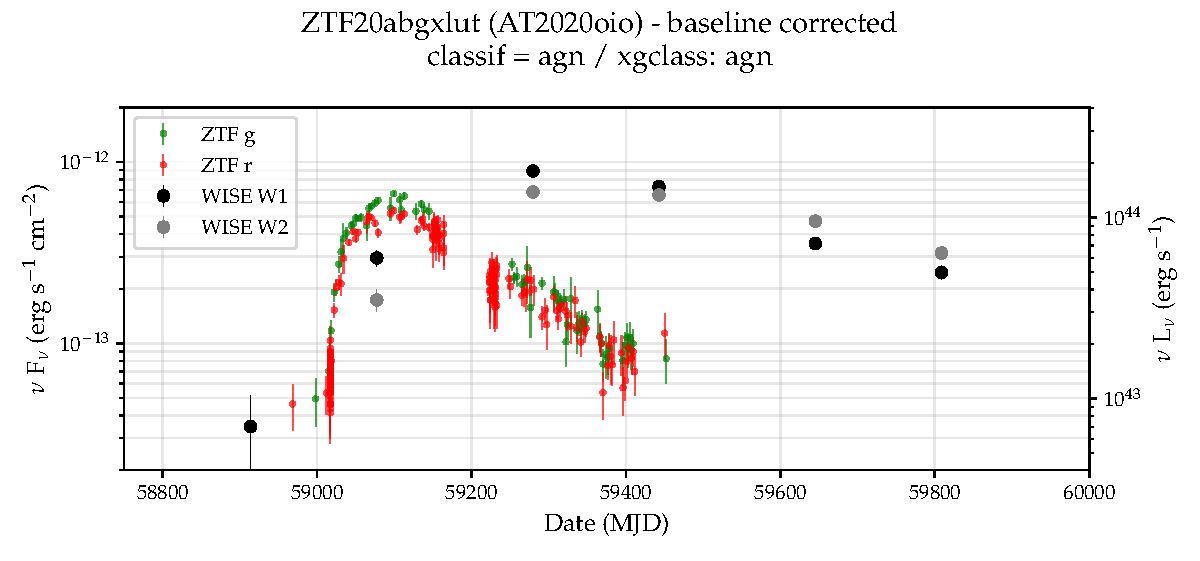
\includegraphics[width=0.4\textwidth]{/Users/simeon/ZTFDATA/nuclear_sample/plots/lightcurves/thumbnails/ZTF20abgxlut.pdf}} & \textbf{\textit{\href{https://ztfnuclear.simeonreusch.com/transient/ZTF20abgxlut}{ZTF20abgxlut}}} & \textbf{0.257} & \textbf{spec.}           & \textbf{AGN}            & \textbf{\textit{\href{https://www.wis-tns.org/object/2020oio}{AT2020oio}}} & \textbf{18.85}             &                                              \\
    \end{tabular}}
\end{table*}


\begin{table*}[t!]
  \resizebox{1.5\textwidth}{!}{%
    \begin{tabular}{c  c  c  c  c  c  c  c}
      \hline
      \textbf{Light curve}                                                                                                                        & \textbf{Transient}                                                                                 & \textbf{z}     & \textbf{z}     & \textbf{Community}      & \textbf{IAU name}                                                            & \textbf{Peak mag.}         & \textbf{Notes}      \\
                                                                                                                                                  &                                                                                                    &                & \textbf{type}  & \textbf{classification} &                                                                              & \textbf{(\textit{g}-band)} &                     \\
      \hline
      \hline
      \parbox[c]{12em}{\includegraphics[width=0.4\textwidth]{/Users/simeon/ZTFDATA/nuclear_sample/plots/lightcurves/thumbnails/ZTF20abhrmri.pdf}} & \textbf{\textit{\href{https://ztfnuclear.simeonreusch.com/transient/ZTF20abhrmri}{ZTF20abhrmri}}}  & ~              & ~              & \textbf{AGN}            & \textbf{\textit{\href{https://www.wis-tns.org/object/2020nnc}{AT2020nnc}}}   & \textbf{19.41}             &                     \\
      \parbox[c]{12em}{\includegraphics[width=0.4\textwidth]{/Users/simeon/ZTFDATA/nuclear_sample/plots/lightcurves/thumbnails/ZTF20ablvwmh.pdf}} & \textbf{\textit{\href{https://ztfnuclear.simeonreusch.com/transient/ZTF20ablvwmh}{ZTF20ablvwmh}}}  & \textbf{0.337} & \textbf{phot.} & \textbf{AGN}            & \textbf{\textit{\href{https://www.wis-tns.org/object/2020xtj}{AT2020xtj}}}   & \textbf{19.36}             &                     \\
      \parbox[c]{12em}{\includegraphics[width=0.4\textwidth]{/Users/simeon/ZTFDATA/nuclear_sample/plots/lightcurves/thumbnails/ZTF20abxtsgg.pdf}} & \textbf{\textit{\href{https://ztfnuclear.simeonreusch.com/transient/ZTF20abxtsgg}{ZTF20abxtsgg}}}  & ~              & ~              & \textbf{Unclassified}   & ~                                                                            & \textbf{19.94}             &                     \\
      \parbox[c]{12em}{\includegraphics[width=0.4\textwidth]{/Users/simeon/ZTFDATA/nuclear_sample/plots/lightcurves/thumbnails/ZTF20acbcfaa.pdf}} & \textit{\href{https://ztfnuclear.simeonreusch.com/transient/ZTF20acbcfaa}{ZTF20acbcfaa}}           & 0.264          & spec.          & CCSN                    & \textit{\href{https://www.wis-tns.org/object/2020usa}{SN2020usa}}            & 18.68                      & \cite{Thevenot2021} \\
      \parbox[c]{12em}{\includegraphics[width=0.4\textwidth]{/Users/simeon/ZTFDATA/nuclear_sample/plots/lightcurves/thumbnails/ZTF20actrcji.pdf}} & \textbf{\textit{\href{https://ztfnuclear.simeonreusch.com/transient/ZTF20actrcji}{ZTF20actrcji}}}  & ~              & ~              & \textbf{Unclassified}   & \textbf{\textit{\href{https://www.wis-tns.org/object/2020abhp}{AT2020abhp}}} & \textbf{17.77}             &                     \\
      \parbox[c]{12em}{\includegraphics[width=0.4\textwidth]{/Users/simeon/ZTFDATA/nuclear_sample/plots/lightcurves/thumbnails/ZTF20acvfraq.pdf}} & \textit{\href{https://ztfnuclear.simeonreusch.com/transient/ZTF20acvfraq}{ZTF20acvfraq}}           & 0.26           & spec.          & AGN                     & \textit{\href{https://www.wis-tns.org/object/2020adpi}{AT2020adpi}}          & 17.9                       & \cite{Hinkle2022}   \\
      \parbox[c]{12em}{\includegraphics[width=0.4\textwidth]{/Users/simeon/ZTFDATA/nuclear_sample/plots/lightcurves/thumbnails/ZTF20acyxxfo.pdf}} & \textbf{\textit{\href{https://ztfnuclear.simeonreusch.com/transient/ZTF20acyxxfo}{ZTF20acyxxfo}} } & \textbf{0.268} & \textbf{phot.} & \textbf{Unclassified}   & \textbf{\textit{\href{https://www.wis-tns.org/object/2020aetz}{AT2020aetz}}} & \textbf{19.6}              &                     \\
      \parbox[c]{12em}{\includegraphics[width=0.4\textwidth]{/Users/simeon/ZTFDATA/nuclear_sample/plots/lightcurves/thumbnails/ZTF21aaekxxf.pdf}} & \textbf{\textit{\href{https://ztfnuclear.simeonreusch.com/transient/ZTF21aaekxxf}{ZTF21aaekxxf}}}  & \textbf{0.26}  & \textbf{phot.} & \textbf{Unclassified}   & \textbf{\textit{\href{https://www.wis-tns.org/object/2021esn}{AT2021esn}}}   & \textbf{20.96}             &                     \\
      \parbox[c]{12em}{\includegraphics[width=0.4\textwidth]{/Users/simeon/ZTFDATA/nuclear_sample/plots/lightcurves/thumbnails/ZTF21aawlhnk.pdf}} & \textit{\href{https://ztfnuclear.simeonreusch.com/transient/ZTF21aawlhnk}{ZTF21aawlhnk}}           & 0.0506         & spec.          & Unclassified            & \textit{\href{https://www.wis-tns.org/object/2019thh}{AT2019thh}}            & 19.36                      & \cite{Velzen2021}   \\
      \hline
    \end{tabular}}
\end{table*}